\documentclass{article}
\usepackage{geometry}
 \geometry{
 top=20mm,
 }
\usepackage[utf8]{inputenc}
\usepackage{listings}
\usepackage{hyperref}
\usepackage{graphicx}
\usepackage{float}
\usepackage{placeins}
\usepackage{subcaption}
\usepackage{cleveref}

\hypersetup{
	colorlinks=true,
	allcolors=blue,
	}
	


\title{COL333 - Assignment 4\\Fuzzy Inference System}
\author{Aman Agrawal (2015CS10210)\\ Suyash Agrawal (2015CS10262)}


\begin{document}

\maketitle

\section{Structure}

The fuzzy inference system has a structure as shown in \cref{fig:structure}.\\
There are $3$ inputs and $1$ output. \\The inputs are
\begin{itemize}
	\item CGPA : It has a range from $[0,10]$
	\item Sports : The number of games played/won. It has a range from $[0,100]$
	\item Co-curricular Activites : The number of certificates won. It has a range from $[0,50]$
\end{itemize}
The output is a Performance Score. It has a range from $[0,10]$

\begin{figure}[H]
 	\centering
	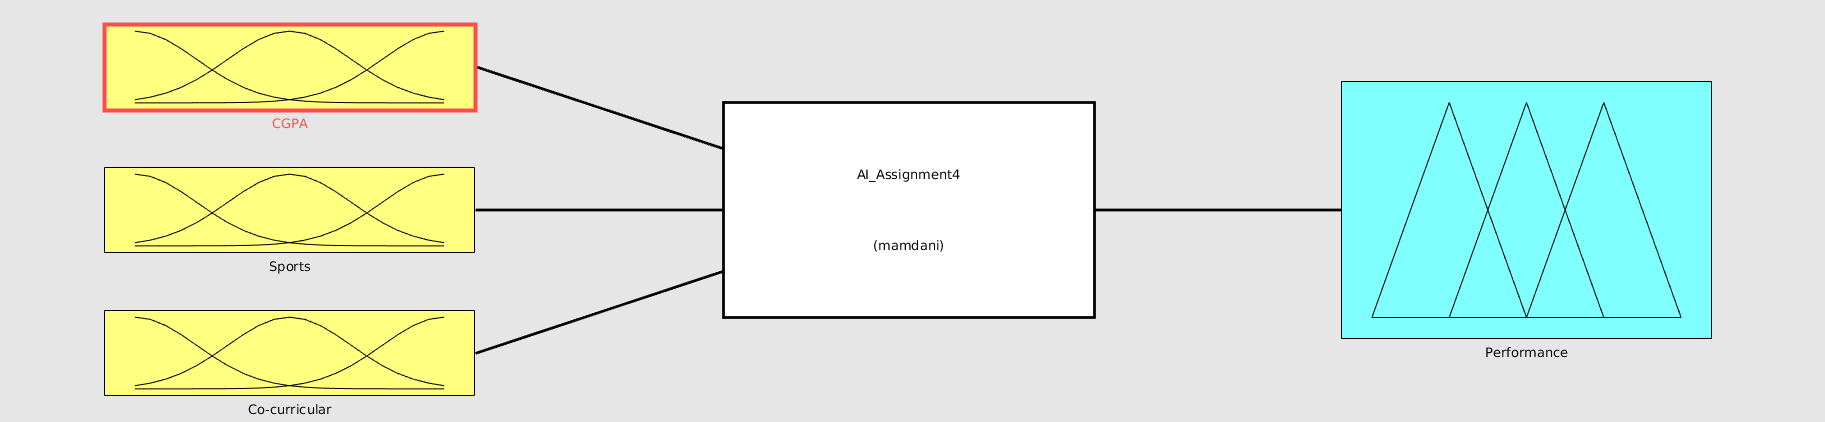
\includegraphics[width=0.8\textwidth,height=0.3\textheight]{imgs/structure.png}
 	\caption{Structure of Fuzzy Inference System\label{fig:structure}}
	\centering
\end{figure}

\section{Membership Functions}
The following membership functions were used for the various inputs and outputs as shown in \cref{fig:membership}
\begin{figure*}
	\centering
	\begin{subfigure}[ht]{0.475\textwidth}
		\centering
		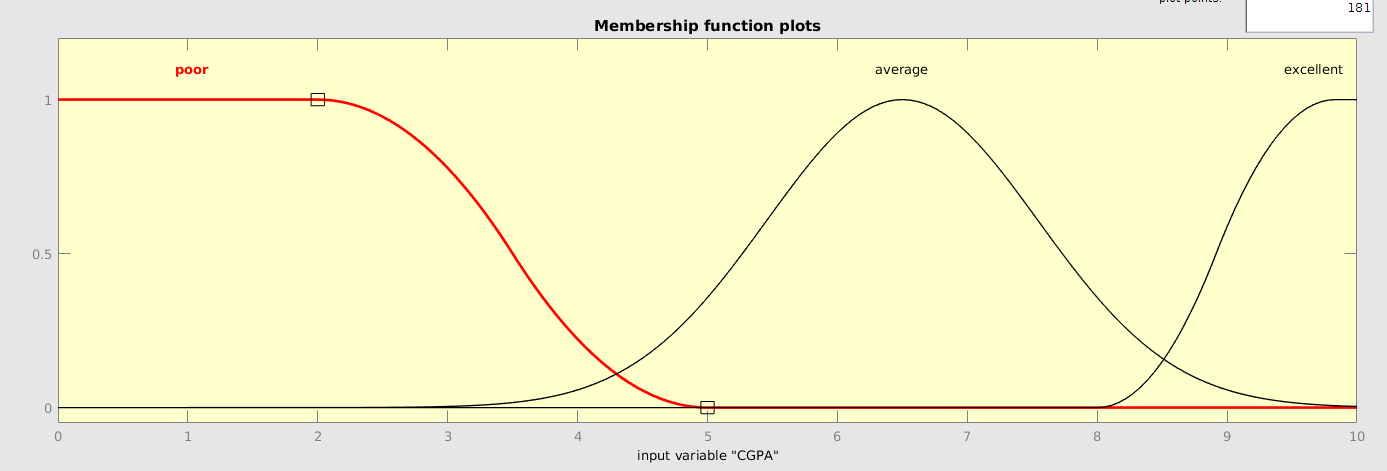
\includegraphics[width=\textwidth,height=0.25\textheight]{imgs/cgpa.png}
		\caption{CGPA\label{fig:cgpa}}    
	\end{subfigure}
	\hfill
	\begin{subfigure}[ht]{0.475\textwidth}  
		\centering 
		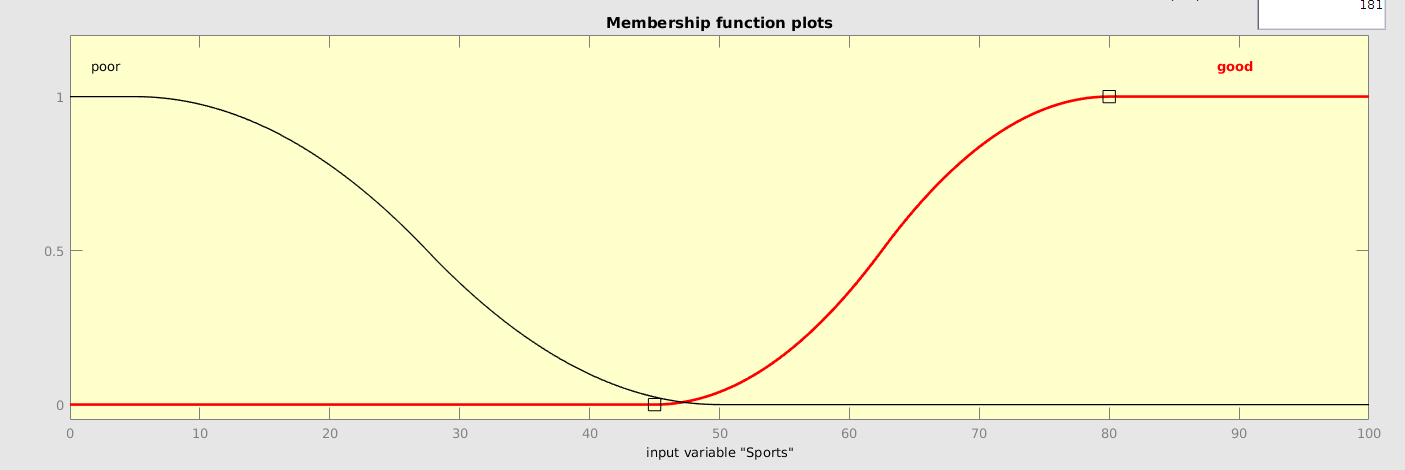
\includegraphics[width=\textwidth,height=0.25\textheight]{imgs/sports.png}
		\caption{Sports\label{fig:sports}}    
	\end{subfigure}
	\vskip\baselineskip
	\begin{subfigure}[ht]{0.475\textwidth}   
		\centering 
		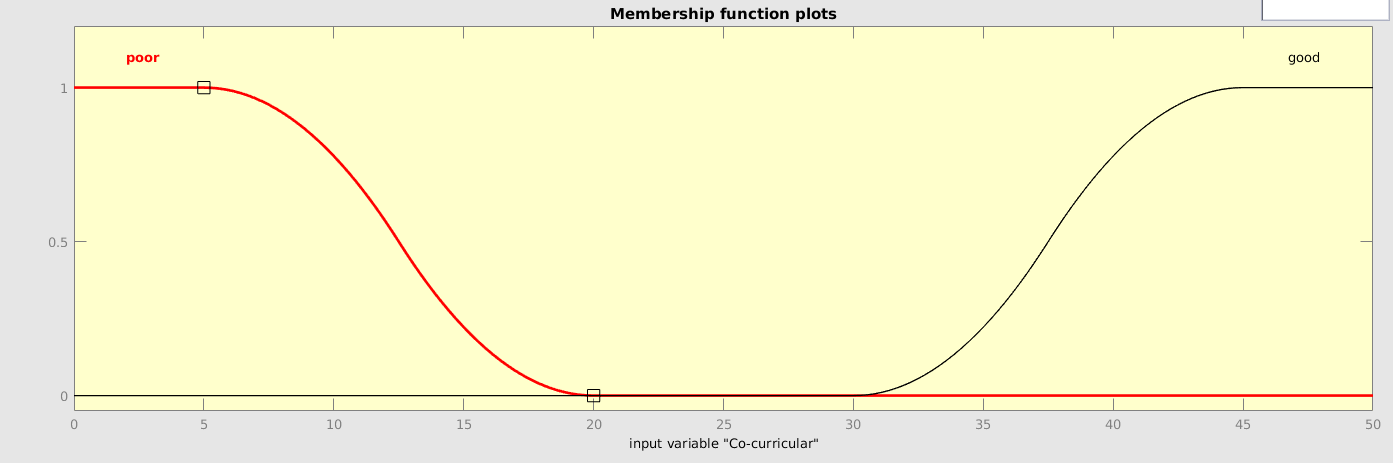
\includegraphics[width=\textwidth,height=0.25\textheight]{imgs/co.png}
		\caption{Co-curricular Activites\label{fig:co}}
	\end{subfigure}
	\quad
	\begin{subfigure}[ht]{0.475\textwidth}   
		\centering 
		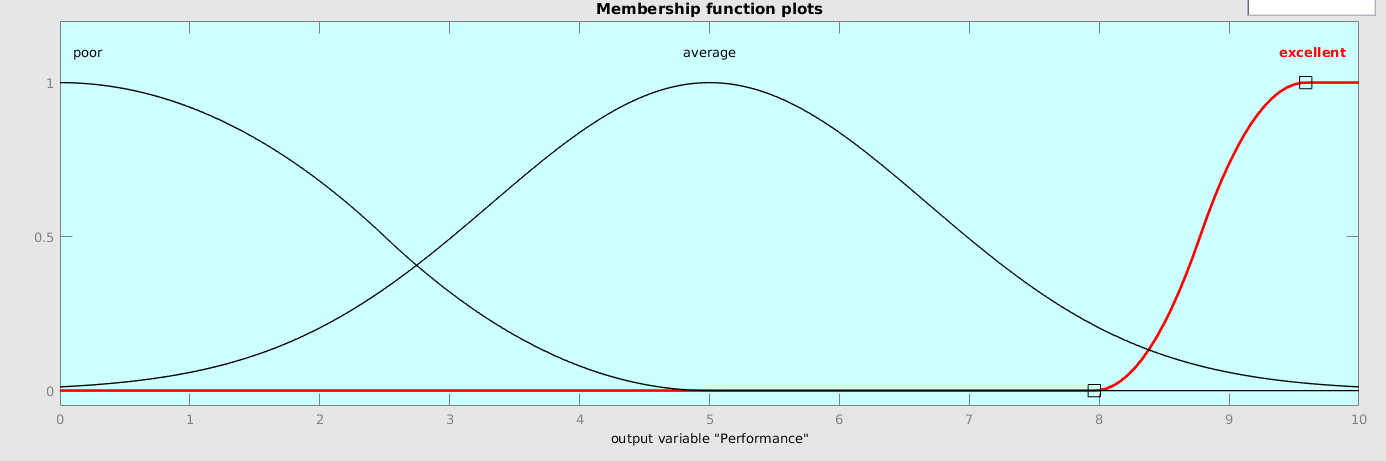
\includegraphics[width=\textwidth,height=0.25\textheight]{imgs/performance.png}
		\caption{Performance\label{fig:performance}}            
	\end{subfigure}
	\caption{Membership Functions for inputs and outputs\label{fig:membership}}
\end{figure*}
\pagebreak

\section{Rules}

The rules used for inference were:

\begin{itemize}

	\item If (CGPA is excellent) then (performance is excellent)
	\item If (CGPA is average) and (Sports is good) and (Co-curricular is good) then (performance is excellent)
	\item If (CGPA is poor) then (performance is poor)
	\item If (CGPA is average) and (Sports is poor) and (Co-curricular is poor) then (performance is average)
	\item If (CGPA is average) and (Sports is not good) and (Co-curricular is good) then (performance is average)
	\item If (CGPA is average) and (Spots is good) and (Co-curricular is not good) then (performance is average)
	
\end{itemize}


\section{Sample Output}

A sample output is shown in the \cref{fig:demo} for the input value of CGPA=9.5, Sports=50, Co-curricular=25.
\\The performance score for this input is 8.84

\begin{figure}[H]
	\centering
   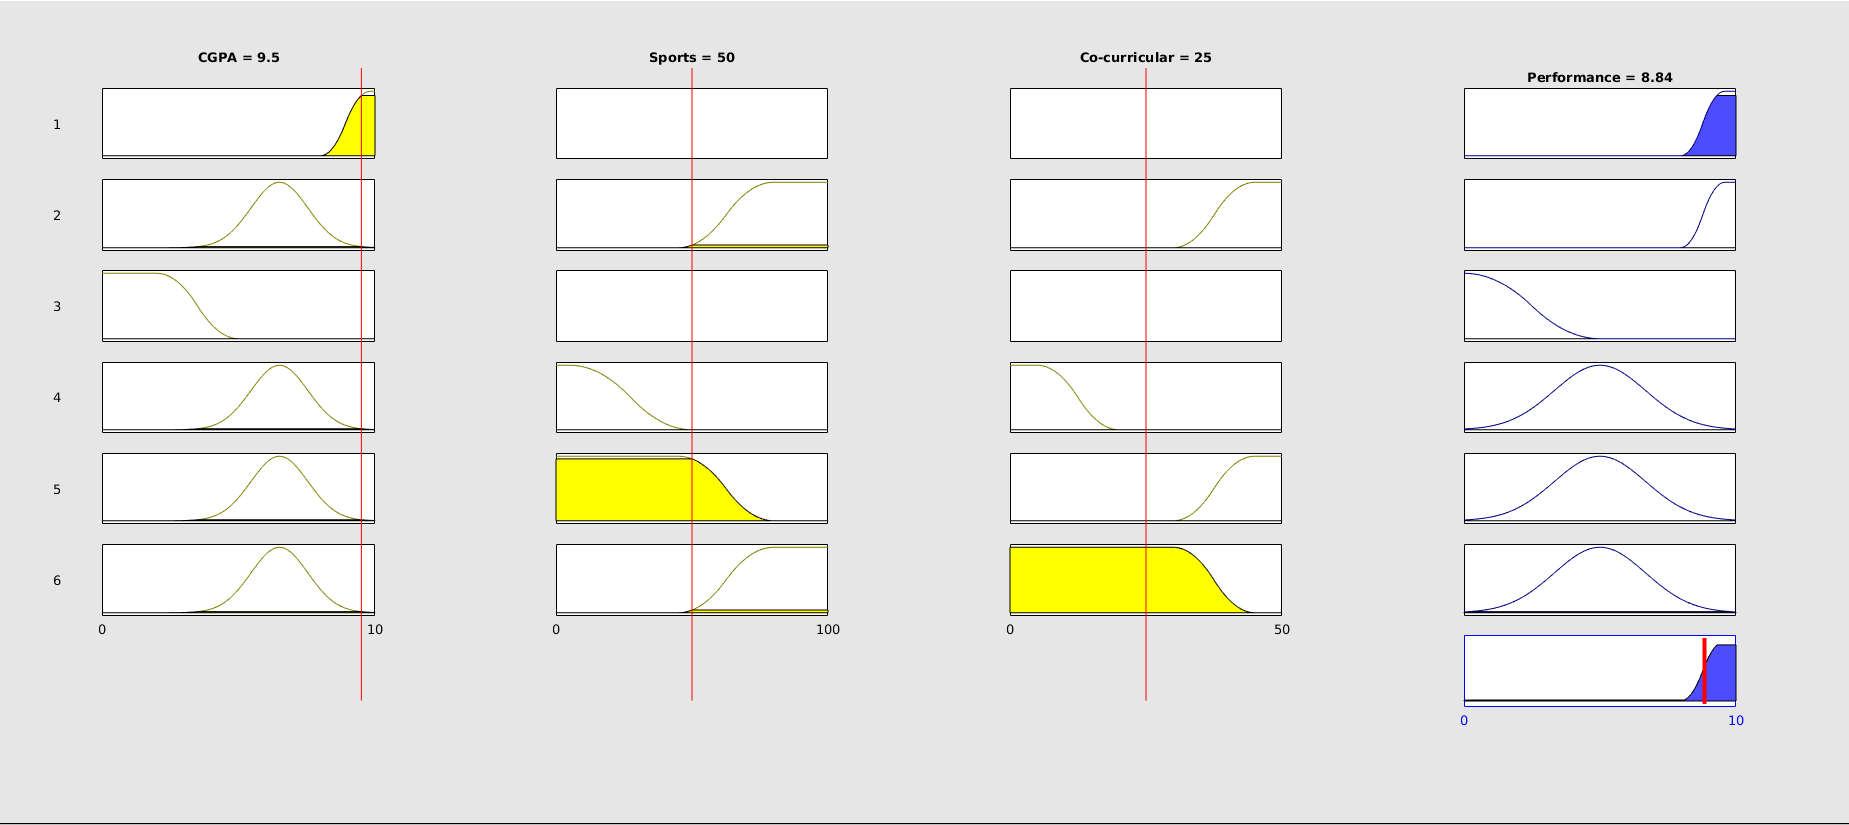
\includegraphics[width=0.8\textwidth,height=0.3\textheight]{imgs/demo.png}
	\caption{Demo for a sample input case\label{fig:demo}}
   \centering
\end{figure}


\end{document}